\chapter{النواقل والعوازل}\label{ch:g4:conductors-insulators}

لماذا تُصنع الأسلاك الكهربائية من معدن --- ثم تُكسى بالبلاستيك؟
ولماذا ينقل جسر \omterm{ex:g3:first-electric-circuit:switch}{القاطعة} الصغير التيارَ بينما يحفظ غلافها أصابعك؟
في السنة الماضية أغلقنا الحلقات؛ وهذه السنة نسأل في أيّ الموادّ
تستطيع الكهرباء أن تسافر أصلًا. والجواب يصنّف كل مادة في صنفين:
نواقل وعوازل.

\section{المختبِر}

\begin{method}[كيف تبني مختبِرًا]\label{met:g4:conductors-insulators:tester}
ابنِ حلقة السنة الماضية --- \omterm{def:g3:first-electric-circuit:battery}{بطارية} وأسلاك \omterm{def:g3:first-electric-circuit:bulb}{ومصباح} --- لكن اترك
فيها فراغًا مقصودًا: طرفَي سلك حرّين، بينهما عرض إصبع.
\begin{enumerate}
  \item المِس الطرفين الحرّين أحدهما بالآخر: يضيء \omterm{def:g3:first-electric-circuit:bulb}{المصباح} ---
        فالمختبِر يعمل؛
  \item ثم اجسر الفراغ بالجسم موضع الاختبار، مع ضغط طرف معدني
        على كل سلك ضغطًا محكمًا؛
  \item وراقب \omterm{def:g3:first-electric-circuit:bulb}{المصباح}: \omterm{def:g1:light-and-shadows:source}{فالضوء} يعني أن الكهرباء عبرت الجسم؛
        والعتمة تعني أنها لم تستطع.
\end{enumerate}
\omterm{def:g3:first-electric-circuit:bulb}{المصباح} يعطي الجواب: فهو يضيء بالضبط حين يُكمل الجسمُ المختبَر
الحلقةَ.
\end{method}

\begin{omfigure}
\begin{tikzpicture}[scale=0.9]
  \draw (0,0) to[battery1, l=بطارية] (0,2.6)
    to[short] (2.2,2.6)
    to[lamp, l=مصباح] (4.4,2.6)
    to[short] (6.0,2.6) -- (6.0,1.7);
  \draw (6.0,0.9) -- (6.0,0) to[short] (0,0);
  \fill (6.0,1.7) circle (1.6pt) node[right, font=\small]
    {~طرف حرّ};
  \fill (6.0,0.9) circle (1.6pt) node[right, font=\small]
    {~طرف حرّ};
  \draw[thick, fill=omMeth, fill opacity=0.4]
    (5.75,0.95) rectangle (6.25,1.65);
  \node[right, font=\small] at (6.6,1.3) {الجسم المختبَر};
\end{tikzpicture}

{\small المختبِر: حلقة سليمة فيها فراغ واحد. وكل ما يجسر الفراغ
هو موضع الاختبار --- \omterm{def:g3:first-electric-circuit:bulb}{والمصباح} يبيّن أيعبره التيار أم لا.}
\end{omfigure}

\section{النواقل والعوازل}

\begin{definition}[الناقل]\label{def:g4:conductors-insulators:conductor}
\emph{الناقل}\index{ناقل} مادة تدع الكهرباء تسافر فيها. وفي
المختبِر يُغلق الناقلُ الجاسر للفراغ الحلقةَ فيضيء \omterm{def:g3:first-electric-circuit:bulb}{المصباح}.
\end{definition}

\begin{definition}[العازل]\label{def:g4:conductors-insulators:insulator}
\emph{العازل}\index{عازل} مادة تحجب الكهرباء. وجسر الفراغ بعازل
يترك الحلقة مفتوحة كما كانت: فيبقى \omterm{def:g3:first-electric-circuit:bulb}{المصباح} معتمًا.
\end{definition}

\begin{example}[صباح من الاختبارات]\label{ex:g4:conductors-insulators:trials}
نتائج مختبِر في صفّ: مشبك ورق فولاذي --- \omterm{def:g1:light-and-shadows:source}{ضوء}. وقطعة نقود ---
\omterm{def:g1:light-and-shadows:source}{ضوء}. ورقاقة ألمنيوم من المطبخ --- \omterm{def:g1:light-and-shadows:source}{ضوء}. ومفتاح --- \omterm{def:g1:light-and-shadows:source}{ضوء}.
ومسطرة بلاستيكية --- عتمة. وقلم خشبي --- عتمة. وكرة زجاجية
--- عتمة. وممحاة مطّاطية --- عتمة. وشريط ورق --- عتمة. والنمط
يقفز إلى العين: فالأجسام التي تضيء \omterm{def:g3:first-electric-circuit:bulb}{المصباح} كلها مصنوعة من
معدن.
\end{example}

\begin{proposition}[المعادن ناقلة]\label{prop:g4:conductors-insulators:metals}
كل المعادن تنقل الكهرباء --- الحديد والنحاس والألمنيوم والذهب،
كلها، ولهذا فاجأتنا انتقائية \omterm{def:g1:magnets:magnet}{المغناطيس} للحديد ولن يفاجئنا
المختبِر أبدًا. وأكثر الأجسام الصلبة اليومية الأخرى ---
البلاستيك والخشب والزجاج والمطّاط والورق والشمع --- عوازل.
\end{proposition}

\begin{remark}[الناقل ليس مغناطيسيًّا]\label{rem:g4:conductors-insulators:notmagnet}
لا تخلط بين موهبتَي المعادن. \omterm{def:g1:magnets:magnet}{فالمغناطيس} لا يختار إلا الحديد
وأسرته؛ أما التيار الكهربائي فأقلّ انتقاءً بكثير ويسافر في
\emph{كل} معدن. ورقاقة الألمنيوم التي أهملت مغناطيسك تحمل
التيار حملًا جميلًا --- لعبتان مختلفتان، وقاعدتان مختلفتان.
\end{remark}

\section{النواقل والعوازل تعمل معًا}

\begin{example}[تشريح سلك]\label{ex:g4:conductors-insulators:wire}
انظر إلى طرف كبل \omterm{def:g3:first-electric-circuit:bulb}{مصباح} حيث يدخل القابس: في الداخل يجري نحاس
لامع --- \omterm{def:g4:conductors-insulators:conductor}{ناقل}، وهو طريق التيار؛ وحوله يلتفّ بلاستيك ملوّن ---
\omterm{def:g4:conductors-insulators:insulator}{عازل}، وهو سياج الطريق. النحاس يقوم بالعمل؛ والبلاستيك يبقي
التيار في الداخل وأصابعك في الخارج. وكل كبل في بيتك يزاوج
بينهما: \omterm{def:g4:conductors-insulators:conductor}{ناقل} داخل \omterm{def:g4:conductors-insulators:insulator}{عازل}.
\end{example}

\begin{omfigure}
\begin{tikzpicture}[scale=0.85]
  \draw[thick, fill=omExo, fill opacity=0.25]
    (0.5,0.35) rectangle (6.5,1.65);
  \draw[thick, fill=omThm, fill opacity=0.45]
    (0.5,0.78) rectangle (7.6,1.22);
  \node[right, font=\small] at (8.35,1.8) {غلاف بلاستيكي: عازل};
  \draw[-Stealth, omExo] (8.3,1.8) -- (6.3,1.55);
  \node[right, font=\small] at (8.35,1.0) {لبّ نحاسي: ناقل};
  \draw[-Stealth, omExo] (8.3,1.0) -- (7.72,1.0);
\end{tikzpicture}

{\small كبل كهربائي مجرّدًا من كسائه: طريق نحاسي للتيار، داخل
سياج بلاستيكي للأمان.}
\end{omfigure}

\begin{omfigure}
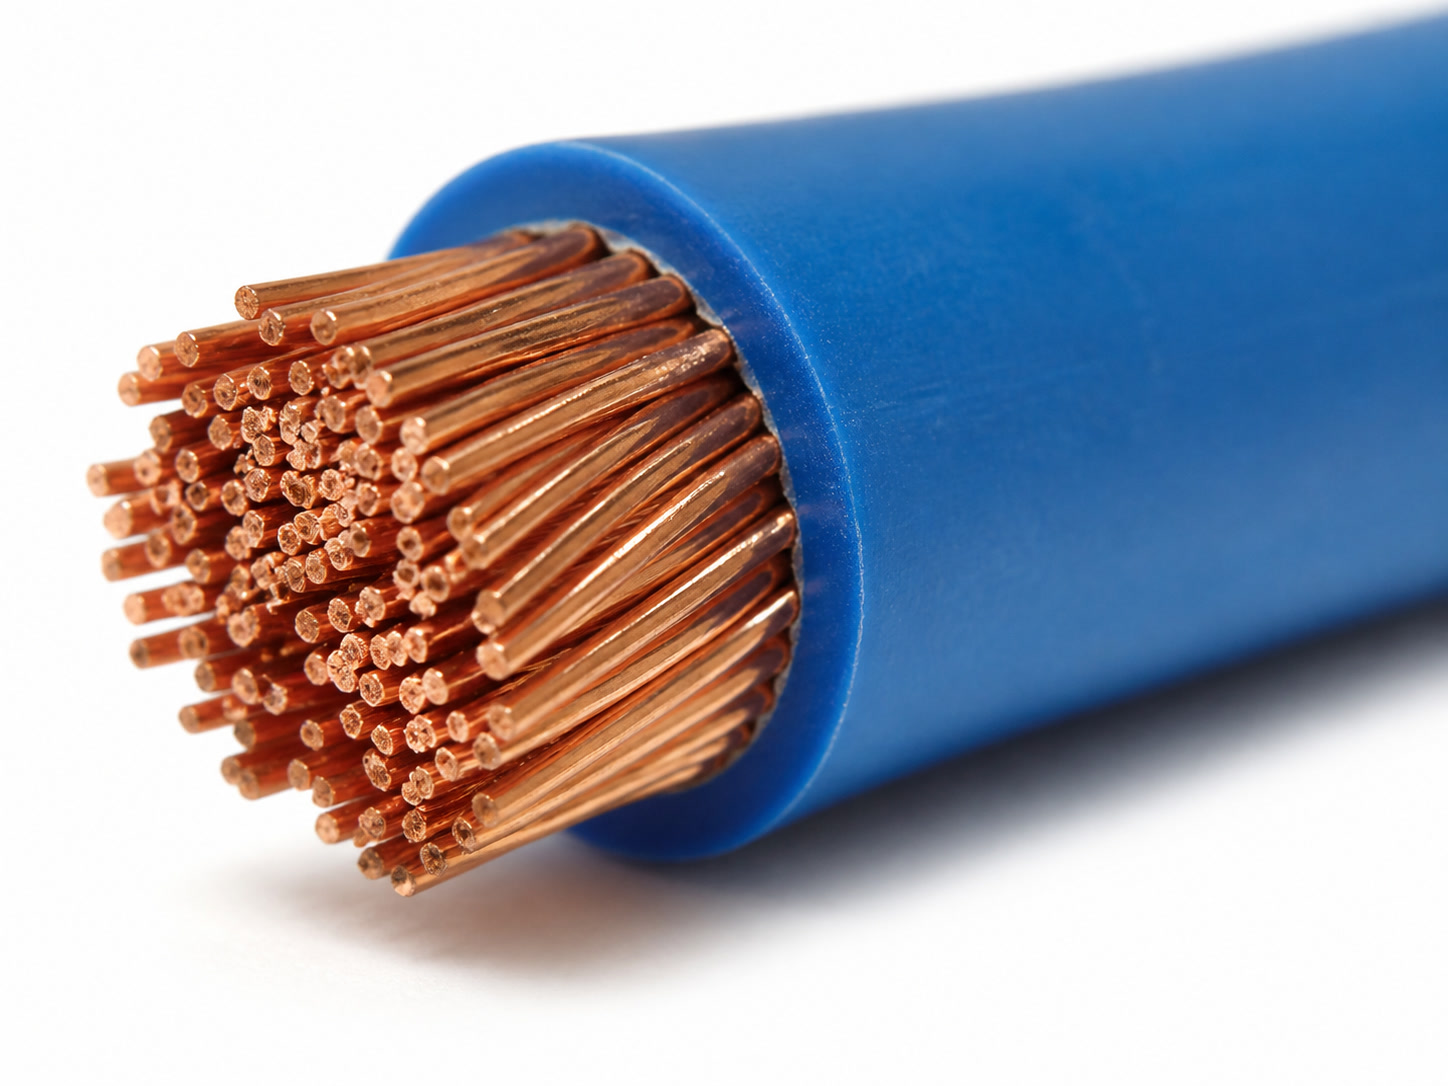
\includegraphics[width=0.5\linewidth]{images/book1/ai/g4-conductors-cable.jpg}

{\small طرف كبل مقطوع، على الحقيقة: خيوط نحاس لامعة --- وهي \omterm{def:g4:conductors-insulators:conductor}{الناقل} --- داخل غلافها البلاستيكي الملوّن --- وهو \omterm{def:g4:conductors-insulators:insulator}{العازل}.}
\end{omfigure}

\begin{example}[قراءة الأشياء اليومية]\label{ex:g4:conductors-insulators:objects}
والآن تشرح تصاميم كثيرة نفسها بنفسها. \omterm{ex:g3:first-electric-circuit:switch}{القاطعة}: جسر معدني (لا بدّ
أن يحمل التيار) في غلاف بلاستيكي (لا يجوز أن يحمله إصبعك).
ومفكّ الكهربائي: نصل فولاذي، ومقبض \omterm{def:g4:conductors-insulators:insulator}{عازل} غليظ. والمأخذ: معدن في
العمق، وبلاستيك في الواجهة. وأبراج التوتر تحمل كبلات معدنية
عارية عاليًا بعيدًا عن المتناول، معلَّقة بأقراص عازلة طويلة حتى
لا يتسرّب التيار إلى البرج.
\end{example}

\begin{remark}[الماء والناس، ولماذا وُضعت القواعد]\label{rem:g4:conductors-insulators:safety}
وهناك \omterm{def:g4:conductors-insulators:conductor}{ناقل} آخر لا بدّ من تسميته: \emph{الأشياء الرطبة} ---
ومنها جلد الإنسان الرطب. ونحن ننقل نقلًا رديئًا، لكن مأخذ الجدار
يدفع دفعًا جبّارًا يجعل الرديء أكثر من كافٍ. وهذا هو السبب
العميق وراء قواعد الأمان التي تعرفها: لا تُدخل شيئًا في مأخذ،
ولا تلمس شيئًا كهربائيًّا بيدين مبتلّتين، وأبعِد مجفّفات الشعر
عن الحمّام. والمختبِر \omterm{def:g3:first-electric-circuit:battery}{بالبطارية} آمن \emph{لأن} دفع \omterm{def:g3:first-electric-circuit:battery}{البطارية}
ضئيل؛ أما المأخذ فلا يغفر شيئًا.
\end{remark}

\section{تمارين}

\begin{exercise}[$\star$]\label{exo:g4:conductors-insulators:1}
ما \omterm{def:g4:conductors-insulators:conductor}{الناقل}؟ وما \omterm{def:g4:conductors-insulators:insulator}{العازل}؟ وأيّهما يضيء \omterm{def:g3:first-electric-circuit:bulb}{مصباح} المختبِر؟
\end{exercise}

\begin{exercise}[$\star$]\label{exo:g4:conductors-insulators:2}
صنّف إلى نواقل وعوازل: ملعقة فولاذية؛ \ فلّينة؛ \ رقاقة مطبخ؛
\ كأس زجاجية؛ \ قطعة نقود نحاسية؛ \ قالب بلاستيكي.
\end{exercise}

\begin{exercise}[$\star$]\label{exo:g4:conductors-insulators:3}
قبل أي تجربة، كيف تتحقّق من أن المختبِر نفسه يعمل؟ ولماذا يهمّ
هذا التحقّق؟
\end{exercise}

\begin{exercise}[$\star$]\label{exo:g4:conductors-insulators:4}
جسم مختبَر يترك \omterm{def:g3:first-electric-circuit:bulb}{المصباح} معتمًا. اذكر سببين محتملين --- واحدًا
يخصّ الجسم، وآخر يخصّ إهمال الاختبار.
\end{exercise}

\begin{exercise}[$\star$]\label{exo:g4:conductors-insulators:5}
لماذا يكون كبل \omterm{def:g3:first-electric-circuit:bulb}{المصباح} نحاسًا من الداخل وبلاستيكًا من الخارج؟
وأيّ عمل تقوم به كل مادة؟
\end{exercise}

\begin{exercise}[$\star$]\label{exo:g4:conductors-insulators:6}
في \omterm{ex:g3:first-electric-circuit:switch}{القاطعة}، أيّ جزء \omterm{def:g4:conductors-insulators:conductor}{ناقل} وأيّ جزء \omterm{def:g4:conductors-insulators:insulator}{عازل}؟ ولماذا تحتاج إلى
الاثنين؟
\end{exercise}

\begin{exercise}[$\star$]\label{exo:g4:conductors-insulators:7}
رقاقة الألمنيوم تهمل \omterm{def:g1:magnets:magnet}{المغناطيس} إهمالًا تامًّا. فهل تضيء \omterm{def:g3:first-electric-circuit:bulb}{مصباح}
المختبِر؟ وأيّ قاعدة تجيب، ومن أيّ خلط تحذّر
\cref{rem:g4:conductors-insulators:notmagnet}؟
\end{exercise}

\begin{exercise}[$\star$]\label{exo:g4:conductors-insulators:8}
القلم خشب فيه سنّ من الغرافيت. ويبقى مختبِر نينو معتمًا عبر
الخشب المطليّ لكنه يضيء ضوءًا خافتًا من سنّ إلى سنّ عبر
الغرافيت المبريّ. فماذا اكتشف نينو عن مادّتَي القلم؟
\end{exercise}

\begin{exercise}[$\star$]\label{exo:g4:conductors-insulators:9}
لماذا تكون مفكّات الكهربائيين وكمّاشاتهم ذات مقابض بلاستيكية
غليظة؟ وأيّ مادة تحمي مَن؟
\end{exercise}

\begin{exercise}[$\star\star$]\label{exo:g4:conductors-insulators:10}
سلسلة قلادة تعطي ``ضوءًا'' في المختبِر؛ وقلادة خرز خشبي تعطي
``عتمة''؛ وقلادة خرز معدني معقود على خيط قطني غليظ تعطي
``عتمة'' أيضًا --- مع أن كل خرزة ناقلة! اشرح النتيجة الثالثة
بتتبّع طريق التيار من خرزة إلى خرزة.
\end{exercise}

\begin{exercise}[$\star\star$]\label{exo:g4:conductors-insulators:11}
لماذا يكون لمس الأشياء الكهربائية بيدين مبتلّتين أخطر بكثير من
لمسها بيدين جافّتين؟ ولماذا يكون المختبِر \omterm{def:g3:first-electric-circuit:battery}{بالبطارية} آمنًا
لتجاربك بينما لا يكون المأخذ آمنًا أبدًا؟ استعمل
\cref{rem:g4:conductors-insulators:safety}.
\end{exercise}
